\documentclass[tikz]{standalone}
\usepackage{amsmath}
\begin{document}
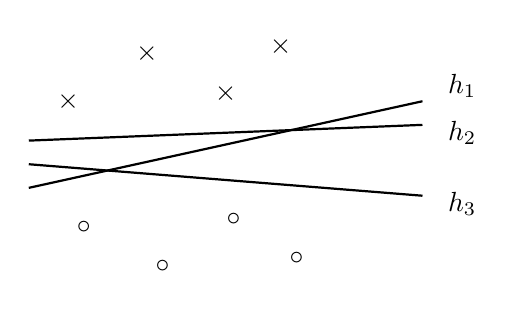
\begin{tikzpicture}[>=stealth,scale=1]

% 数据点（X 类）
\node at (-2,1.2) {$\times$};
\node at (-1,1.8) {$\times$};
\node at (0.0,1.3) {$\times$};
\node at (0.7,1.9) {$\times$};

% 数据点（O 类）
\node at (-1.8,-0.4) {$\circ$};
\node at (-0.8,-0.9) {$\circ$};
\node at (0.1,-0.3) {$\circ$};
\node at (0.9,-0.8) {$\circ$};

% 三条线性分类器（都给出相同分类）
\begin{scope}[shift={(0,0.3)}]
    \draw[thick] (-2.5,0.4) -- (2.5,0.6);    % h1
\draw[thick] (-2.5,0.1) -- (2.5,-0.3);    % h2
\draw[thick] (-2.5,-0.2) -- (2.5,0.9);   % h3
\end{scope}


% 右侧标记 h1, h2, h3

\node[right] at (2.7,1.4) {$h_1$};


\node[right] at (2.7,0.8) {$h_2$};


\node[right] at (2.7,-0.1) {$h_3$};

\end{tikzpicture}
\end{document}